
The fact that the square of every real number is nonnegative shows that the equation $x^{2} + 1 = 0$ has no real root; in other words, there is no real number $u$ such that $u^{2} = -1$. So the set of real numbers is inadequate for finding all roots of all polynomials. This kind of problem arises with other number systems as well. The set of integers contains no solution of the equation $3x + 2 = 0$, and the rational numbers had to be invented to solve such 
equations. But the set of rational numbers is also incomplete because, 
for example, it contains no root of the polynomial $x^{2} - 2$. Hence the real numbers were invented. In the same way, the set of 
complex numbers was invented, which contains all real numbers together 
with a root of the equation $x^{2} + 1 = 0$. However, the process ends here: the complex numbers have the property that \textit{every} polynomial with complex coefficients has a (complex) root. This fact is known as the fundamental theorem of algebra.\index{complex number!fundamental theorem of algebra}\index{fundamental theorem of algebra}\index{polynomials!root}\index{root!of polynomials}


One pleasant aspect of the complex 
numbers is that, whereas describing the real numbers in terms of the 
rationals is a rather complicated business, the complex numbers are 
quite easy to describe in terms of real numbers. Every \textbf{complex number} has the form\index{complex number!form}
\begin{equation*}
a + bi
\end{equation*}
where $a$ and $b$ are real numbers, and $i$ is a root of the polynomial $x^{2} + 1$. Here $a$ and $b$ are called the \textbf{real part}\index{real parts}\index{complex number!real part} and the \textbf{imaginary part}\index{complex number!imaginary part}\index{imaginary parts} of the complex number, respectively. The real numbers are now regarded as special complex numbers of the form $a + 0i = a$, with zero imaginary part. The complex numbers of the form $0 + bi = bi$ with zero real part are called \textbf{pure imaginary} numbers\index{complex number!pure imaginary numbers}\index{pure imaginary numbers}. The complex number $i$ itself is called the \textbf{imaginary unit}\index{complex number!imaginary unit}\index{imaginary unit} and is distinguished by the fact that
\begin{equation*}
i^2 = -1 
\end{equation*}
As the terms \textit{complex} and \textit{imaginary}
 suggest, these numbers met with some resistance when they were first 
used. This has changed; now they are essential in science and 
engineering as well as mathematics, and they are used extensively. The 
names persist, however, and continue to be a bit misleading: These 
numbers are no more ``\textit{complex}'' than the real numbers, and the number $i$ is no more ``\textit{imaginary}'' than $-1$.


Much as for polynomials, two complex numbers are declared to be \textbf{equal}\index{complex number!equal}\index{equal!complex number} if and only if they have the same real parts and the same imaginary parts. In symbols,
\begin{equation*}
a+bi = a^{\prime} + b^{\prime} i \quad \mbox{ if and only if } a = a^{\prime} \mbox{ and } b = b^{\prime} 
\end{equation*}
The addition and subtraction of complex numbers is accomplished by adding and subtracting real and imaginary parts:\index{complex number!addition}\index{addition!complex number}\index{complex number!subtraction}\index{subtraction!complex number}
\begin{align*}
(a+bi) + (a^{\prime} + b^{\prime}i) & = (a + a^{\prime}) + (b + b^{\prime})i\\ 
(a+bi) - (a^{\prime} + b^{\prime}i) & = (a - a^{\prime}) + (b - b^{\prime})i
\end{align*}
This is analogous to these operations for linear polynomials $a + bx$ and $a^{\prime} + b^{\prime}x$, and the multiplication of complex numbers is also analogous with one difference: $i^{2} = -1$. The definition is\index{complex number!multiplication}
\begin{equation*}
(a+bi)(a^{\prime} + b^{\prime}i) = (a a^{\prime} - b b^{\prime}) + (a b^{\prime} + b a^{\prime})i 
\end{equation*}
With these definitions of equality, addition, and multiplication, the complex numbers \textit{satisfy all the basic arithmetical axioms adhered to by the real numbers} (the verifications are omitted). One consequence of this is that they can be manipulated in the obvious fashion, except that $i^{2}$ is replaced by $-1$ wherever it occurs, and the rule for equality must be observed.


\begin{example}{}{033865}
If $z = 2 - 3i$ and $w = -1 + i$, write each of the following in the form $a + bi$: $z + w$, $z - w$, $zw$, $\frac{1}{3}z$, and $z^{2}$.


\begin{solution}
\begin{align*}
z+w & = (2-3i) + (-1+i) = (2-1) + (-3+1)i = 1-2i \\
z-w & = (2-3i) - (-1+i) = (2+1) + (-3-1)i = 3-4i \\ 
zw &= (2-3i)(-1+i) = (-2-3i^2) + (2+3)i = 1+5i \\
\frac{1}{3}z &= \frac{1}{3}(2-3i) = \frac{2}{3}-i \\
z^2 &=(2-3i)(2-3i) = (4+9i^2) + (-6-6)i = -5-12i 
\end{align*}
\end{solution}
\end{example}

\begin{example}{}{033872}
Find all complex numbers $z$ such as that $z^{2} = i$.


\begin{solution}
  Write $z = a + bi$; we must determine $a$ and $b$. Now $z^{2} = (a^{2} - b^{2}) + (2ab)i$, so the condition $z^{2} = i$ becomes
\begin{equation*}
(a^2 - b^2) + (2ab)i = 0+i
\end{equation*}
Equating real and imaginary parts, we find that $a^{2} = b^{2}$ and $2ab = 1$. The solution is $a = b = \pm \frac{1}{\sqrt{2}}$, so the complex numbers required are $z = \frac{1}{\sqrt{2}} + \frac{1}{\sqrt{2}}i$  and  $z = -\frac{1}{\sqrt{2}} - \frac{1}{\sqrt{2}}i$.
\end{solution}
\end{example}

As for real numbers, it is possible to divide by every nonzero complex number $z$. That is, there exists a complex number $w$ such that $wz = 1$. As in the real case, this number $w$ is called the \textbf{inverse}\index{complex number!inverse}\index{inverses!complex number} of $z$ and is denoted by $z^{-1}$ or $\frac{1}{z}$. Moreover, if $z = a + bi$, the fact that $z \neq 0$ means that $a \neq 0$ or $b \neq 0$. Hence $a^{2} + b^{2} \neq 0$, and an explicit formula for the inverse is
\begin{equation*}
\frac{1}{z} = \frac{a}{a^2 + b^2} - \frac{b}{a^2+b^2}{i}
\end{equation*}
In actual calculations, the work is 
facilitated by two useful notions: the conjugate and the absolute value 
of a complex number.\index{absolute value!complex number}\index{complex number!absolute value} The next example illustrates the technique.

\newpage

\begin{example}{}{033897}
Write $\frac{3+2i}{2+5i}$ in the form $a + bi$.


\begin{solution}
  Multiply top and bottom by the complex number $2 - 5i$ (obtained from the denominator by negating the imaginary part). The result is
\begin{equation*}
\frac{3+2i}{2+5i} = \frac{(2-5i)(3+2i)}{(2-5i)(2+5i)} = \frac{(6+10)+(4-15)i}{2^2-(5i)^2} = \frac{16}{29} - \frac{11}{29} i 
\end{equation*}
Hence the simplified form is $\frac{16}{29} - \frac{11}{29} i $, as required.
\end{solution}
\end{example}

The key to this technique is that the product $(2 - 5i)(2 + 5i) = 29$ in the denominator turned out to be a \textit{real} number. The situation in general leads to the following notation: If $z = a + bi$ is a complex number, the \textbf{conjugate}\index{complex number!conjugate}\index{conjugate} of $z$ is the complex number, denoted $\overline{z}$, given by
\begin{equation*}
\overline{z} = a-bi \quad \mbox{ where } z = a+bi
\end{equation*} 
Hence $\overline{z}$ is obtained from $z$ by negating the imaginary part. Thus $\overline{(2+3i)} = 2-3i$ and  $\overline{(1-i)} = 1+i$. If we multiply $z = a + bi$ by $\overline{z}$, we obtain
\begin{equation*}
z \overline{z} = a^2 + b^2 \quad \mbox{ where } z = a+bi
\end{equation*}

The real number $a^{2} + b^{2}$ is always nonnegative, so we can state the following definition: The \textbf{absolute value}\index{absolute value!complex number}\index{complex number!absolute value} or \textbf{modulus}\index{modulus}\index{complex number!modulus} of a complex number $z = a + bi$, denoted by $|z|$, is the positive square root $\sqrt{a^2 + b^2}$; that is,
\begin{equation*}
|z| = \sqrt{a^2 + b^2} \quad \mbox{ where } z = a+bi
\end{equation*}
For example, $| 2-3i| = \sqrt{2^2 + (-3)^2} = \sqrt{13}$
 and $| 1+i| = \sqrt{1^2 + 1^2} = \sqrt{2}$.


Note that if a real number $a$ is viewed as the complex number $a + 0i$, its absolute value (as a complex number) is $|a| = \sqrt{a^2}$, which agrees with its absolute value as a \textit{real} number.


With these notions in hand, we can describe the technique applied in Example~\ref{exa:033897}  as follows: When converting a quotient $\frac{z}{w}$
 of complex numbers to the form $a + bi$, multiply top and bottom by the conjugate  $\overline{w}$ of the denominator.

The following list contains the most important properties of conjugates and absolute values. Throughout, $z$ and $w$ denote complex numbers.
\begin{equation*}
\def\arraystretch{1.5}
\begin{array}{llcll}
C1. & \overline{z \pm w} = \overline{z} \pm \overline{w} & \quad & C7. & \frac{1}{z} = \frac{1}{|z|^2}\overline{z} \\
C2. & \overline{zw} = \overline{z}~\overline{w} & \quad & C8. & |z| \geq 0 \mbox{ for all complex numbers } z \\
C3. & \overline{\left(\frac{z}{w}\right)} = \frac{\overline{z}}{\hspace{0.05em}\overline{w}\hspace{0.05em}} & \quad & C9. & |z| = 0 \mbox{ if and only if } z=0 \\
C4. & \overline{(\overline{z})} = z & \quad & C10. & |zw| = |z||w| \\
C5. & z \mbox{ is real if and only if } \overline{z} =z  & \quad & C11. & |\frac{z}{w}| = \frac{|z|}{|w|} \\
C6. & z\overline{z} = |z|^2 & \quad & C12. & |z+w| \leq |z|+|w| \mbox{ (\textbf{triangle inequality})}\index{complex number!triangle inequality}\index{triangle!inequality}\index{triangle inequality} \\
\end{array}
\end{equation*}
All these properties (except property C12) can (and should) be verified by the reader for arbitrary complex numbers $z = a + bi$ and $w = c + di$. They are not independent; for example, property C10 follows from properties C2 and C6.

The triangle inequality, as its name 
suggests, comes from a geometric representation of the complex numbers 
analogous to identification of the real numbers with the points of a 
line. The representation is achieved as follows:

\begin{wrapfigure}{l}{5cm}
	\centering
	
\begin{tikzpicture}
%set up of axis environment
\begin{axis}[disabledatascaling,
	clip mode=individual, 
    width=5cm, 
    height=5cm, 
    xlabel={$x$}, 
    ylabel={$y$}, 
    axis lines=middle, 
    xtick={1}, 
    ytick={1}, 
    xticklabels={$1$}, 
    yticklabels={$i$}, 
    every axis x label/.style={
      at={(ticklabel* cs:1.05)},
      anchor=west,font=\footnotesize
    },
    every axis y label/.style={
      at={(ticklabel* cs:1.05)},
      anchor=south,font=\footnotesize
    },
	tick label style={font=\footnotesize},
    domain=-5:5, 
    samples=100, 
    xmin=-2, 
    xmax=5, 
    ymin=-4, 
    ymax=5]
\draw[thick](0,0)--(2,3);
\draw[dkbluevect,thick,dashed](0,3)--(2,3);
\draw[dkbluevect,thick,dashed](2,3)--(2,-3);
\fill (0,3) circle (2pt);
\fill (0,0) circle (2pt);
\fill (2,3) circle (2pt);
\fill (2,0) circle (2pt);
\fill (2,-3) circle (2pt);
\node[below,font=\footnotesize] at (3,-3){$(a,-b)=a-bi$};
\node[below left,font=\footnotesize] at (0,0){$0$};
\node[left,font=\footnotesize] at (0,3){$(0,b)=bi$};
\node[above,font=\footnotesize] at (2.5,3){$(a,b)=a+bi$};
\node[above right,font=\footnotesize] at (2,0){$(a,0)=a$};
\end{axis}
\end{tikzpicture}

	\caption{\label{fig:033934}}
\end{wrapfigure}

Introduce a rectangular coordinate system in the plane (Figure~\ref{fig:033934}), and identify the complex number $a + bi$ with the point $(a, b)$. When this is done, the plane is called the \textbf{complex plane}\index{complex number!in complex plane}\index{complex plane}. Note that the point $(a, 0)$ on the $x$ axis now represents the \textit{real} number $a = a + 0i$, and for this reason, the $x$ axis is called the \textbf{real axis}\index{real axis}\index{complex number!real axis}. Similarly, the $y$ axis is called the \textbf{imaginary axis}\index{complex number!imaginary axis}\index{imaginary axis}. The identification $(a, b) = a + bi$ of the geometric point $(a, b)$ and the complex number $a + bi$ will be used in what follows without comment. For example, the origin will be referred to as $0$.

This representation of the complex 
numbers in the complex plane gives a useful way of describing the 
absolute value and conjugate of a complex number $z = a + bi$. The absolute value $|z| = \sqrt{a^2+b^2}$
 is just the distance from $z$ to the origin. This makes properties C8 and C9 quite obvious. The conjugate $\overline{z} = a-bi$ of $z$ is just the reflection of $z$ in the real axis ($x$ axis), a fact that makes properties C4 and C5 clear.


Given two complex numbers $z_{1} = a_{1} + b_{1}i = (a_{1}, b_{1})$ and $z_{2} = a_{2} + b_{2}i = (a_{2}, b_{2})$, the absolute value of their difference
\begin{equation*}
|z_1 - z_2| = \sqrt{(a_1-a_2)^2 + (b_1 - b_2)^2}
\end{equation*}
is just the distance between them. This gives the \textbf{complex distance formula}\index{complex distance formula}:

\begin{wrapfigure}[11]{l}{5cm}
        \vspace*{-2em}
	\centering
	
\begin{tikzpicture}
%set up of axis environment
\begin{axis}[disabledatascaling,
	clip mode=individual, 
    width=5cm, 
    height=5cm, 
    xlabel={$x$}, 
    ylabel={$y$}, 
    axis lines=middle, 
    xtick=\empty, 
    ytick=\empty, 
    xticklabels=\empty, 
    yticklabels=\empty, 
    every axis x label/.style={
      at={(ticklabel* cs:1.05)},
      anchor=west,font=\footnotesize
    },
    every axis y label/.style={
      at={(ticklabel* cs:1.05)},
      anchor=south,font=\footnotesize
    },
	 domain=-5:5, 
    samples=100, 
    xmin=-2, 
    xmax=5, 
    ymin=-1, 
    ymax=5]
\draw[dkgreenvect,thick](0,0)--(3,2);
\draw[dkgreenvect,thick](3,2)--(-1,4);
\draw[dkgreenvect,thick](-1,4)--(0,0);
\fill[black] (0,0) circle (2pt);
\fill[black] (3,2) circle (2pt);
\fill[black] (-1,4) circle (2pt);
\node[below left,font=\footnotesize] at (0,0){$0$};
\node[font=\footnotesize] at (3,1){$|w|$};
\draw[thin](2,1.33)--(2.5,1);
\node[right,font=\footnotesize] at (3,2){$w$};
\node[font=\footnotesize] at (3,4){$|(z+w)-w|=|z|$};
\draw[thin](1.5,2.75)--(2,3.5);
\node[above left,font=\footnotesize] at (-0.8,3.9){$z+w$};
\draw[thin](-0.6,2.4)--(-1,1.9);
\node[font=\footnotesize] at (-2,2){$|z+w|$};
\end{axis}
\end{tikzpicture}

	\caption{\label{fig:033953}}
\end{wrapfigure}

\begin{equation*}
|z_1 - z_2| \mbox{ is the distance between } z_1 \mbox{ and } z_2 
\end{equation*}

This useful fact yields a simple verification of the triangle inequality, property C12. Suppose $z$ and $w$ are given complex numbers. Consider the triangle in Figure~\ref{fig:033953} whose vertices are $0$, $w$, and $z + w$. The three sides have lengths $|z|$, $|w|$, and $|z + w|$ by the complex distance formula, so the inequality
\begin{equation*}
|z+w| \leq |z| + |w|
\end{equation*}
expresses the obvious geometric fact that the sum of the lengths of two 
sides of a triangle is at least as great as the length of the third 
side.

The representation of complex numbers 
as points in the complex plane has another very useful property: It 
enables us to give a geometric description of the sum and product of two
 complex numbers. To obtain the description for the sum, let
\begin{align*}
z & = a+bi = (a,b) \\
w & = c+di = (c,d)
\end{align*}\index{complex number!regular representation}\index{complex number!product}\index{product!complex number}

\begin{wrapfigure}[6]{l}{5cm}
        \vspace*{-5em}
        \vspace*{-4em}
	\centering
	
\begin{tikzpicture}
%set up of axis environment
\begin{axis}[disabledatascaling,
	clip mode=individual, 
    width=5cm, 
    height=5cm, 
    xlabel={$x$}, 
    ylabel={$y$}, 
    axis lines=middle, 
    xtick=\empty, 
    ytick=\empty, 
    xticklabels=\empty, 
    yticklabels=\empty, 
    every axis x label/.style={
      at={(ticklabel* cs:1.05)},
      anchor=west,font=\footnotesize
    },
    every axis y label/.style={
      at={(ticklabel* cs:1.05)},
      anchor=south,font=\footnotesize
    },
	 domain=-5:5, 
    samples=100, 
    xmin=-1, 
    xmax=6, 
    ymin=-1, 
    ymax=5]
\draw[dkgreenvect,thick](0,0)--(4,1);
\draw[dkgreenvect,thick](4,1)--(5,4);
\draw[dkgreenvect,thick](5,4)--(1,3);
\draw[dkgreenvect,thick](1,3)--(0,0);
\fill[black] (0,0) circle (2pt);
\fill[black] (4,1) circle (2pt);
\fill[black] (5,4) circle (2pt);
\fill[black] (1,3) circle (2pt);
\node[below right,font=\footnotesize] at (0,0){$0=(0,0)$};
\node[right,font=\footnotesize] at (4,1){$w=(c,d)$};
\node[above,font=\footnotesize] at (5,4){$z+w=(a+c,b+d)$};
\node[right,font=\footnotesize] at (1,2.75){$z=(a,b)$};
\end{axis}
\end{tikzpicture}

	\caption{\label{fig:033957}}
\end{wrapfigure}


\noindent denote two complex numbers. We claim that the four points $0$, $z$, $w$, and $z + w$ form the vertices of a parallelogram. In fact, in Figure~\ref{fig:033957} the lines from $0$ to $z$ and from $w$ to $z + w$ have slopes
\begin{equation*}
\frac{b-0}{a-0} = \frac{b}{a} \quad \mbox{ and } \quad \frac{(b+d)-d}{(a+c)-c} = \frac{b}{a}
\end{equation*}
respectively, so these lines are parallel. (If it happens that $a = 0$, then both these lines are vertical.) Similarly, the lines from $z$ to $z + w$ and from $0$ to $w$ are also parallel, so the figure with vertices $0$, $z$, $w$, and $z + w$ is indeed a parallelogram. Hence, the complex number $z + w$ can be obtained geometrically from $z$ and $w$ by \textit{completing} the parallelogram. This is sometimes called the \textbf{parallelogram law}\index{complex number!parallelogram law}\index{complex number!sum}\index{sum!complex number}\index{parallelogram!law}
 of complex addition. Readers who have studied mechanics will recall 
that velocities and accelerations add in the same way; in fact, these 
are all special cases of \textit{vector} addition.\index{addition!vector addition}\index{vector addition}

\subsection*{Polar Form}
\begin{wrapfigure}{l}{5cm}
	\centering
	
\begin{tikzpicture}
\begin{axis}[disabledatascaling, 
	clip mode=individual, 
    width=5cm, 
    height=5cm, 
    xlabel={$x$}, 
    ylabel={$y$}, 
    axis lines=middle, 
    xtick={-5,-4,...,5}, 
    ytick={-5,-4,...,5}, 
    xticklabels=\empty, 
    yticklabels=\empty, 
    every axis x label/.style={
      at={(ticklabel* cs:1.05)},
      anchor=west,
    },
    every axis y label/.style={
      at={(ticklabel* cs:1.05)},
      anchor=south,
    },
    domain=-5:5, 
    samples=100, 
    xmin=-1.5, 
    xmax=1.5, 
    ymin=-1.5, 
    ymax=1.5]
\draw[dkgreenvect,thick] (0,0) circle (1); 
\draw[thick,-latex] (0.5,0) arc [start angle=0,end angle=45,radius=0.5] node [right, text=black,font=\footnotesize,midway]{$\theta$};
\draw[thick](0,0)--(1,1);
\fill[black] (1,0) circle (1.5pt);
\fill[black] (0,1) circle (1.5pt);
\fill[black] (-1,0) circle (1.5pt);
\fill[black] (0,-1) circle (1.5pt);
\fill[black] (0.707,0.707) circle (1.5pt);
\node[below left,font=\footnotesize] at (0,0){$0$};
\node[below right,font=\footnotesize] at (1,0){$1$};
\node[above right,font=\footnotesize] at (0,1){$i$};
\node[above left,font=\footnotesize] at (-1,0){$-1$};
\node[below right,font=\footnotesize] at (0,-1){$-i$};
\node[below left,font=\footnotesize] at (0,0){$0$};
\draw[thick,latex-latex] (1.15,0) arc [start angle=0,end angle=45,radius=1.15];
\node[font=\footnotesize,align=center] at (1.5,1.25){Radian \\ measure\\ of $\theta$};
\draw[thin,-latex] (1.5,0.65)--(1.2,0.5);
\node[font=\footnotesize,align=center] at (-1.25,1.25){Unit\\circle};
\draw[thin,-latex] (-1.15,0.85)--(-0.85,0.65);
\node[above,font=\footnotesize] at (0.3535,0.3535){$1$};
\node[above,font=\footnotesize] at (0.707,0.707){$P$};
\end{axis} 
\end{tikzpicture}

	\caption{\label{fig:033966}}
\end{wrapfigure}
\index{complex number!polar form}\index{polar form}

The geometric description of what 
happens when two complex numbers are multiplied is at least as elegant 
as the parallelogram law of addition, but it requires that the complex 
numbers be represented in polar form. Before discussing this, we pause 
to recall the general definition of the trigonometric functions sine and
 cosine. An angle $\theta$ in the complex plane is in \textbf{standard position}\index{angles!standard position}\index{standard position} if it is measured counterclockwise from the positive real axis as indicated in Figure~\ref{fig:033966}.
 Rather than using degrees to measure angles, it is more natural to use 
radian measure. This is defined as follows: The circle with its centre 
at the origin and radius $1$ (called the \textbf{unit circle}\index{unit circle}\index{angles!unit circle}) is drawn in Figure~\ref{fig:033966}. It has circumference $2\pi$, and the \textbf{radian measure}\index{angles!radian measure}\index{radian measure} of $\theta$ is the length of the arc on the unit circle counterclockwise from $1$ to the point $P$ on the unit circle determined by $\theta$. Hence $90^{\circ} = \frac{\pi}{2}$, $45^{\circ}  = \frac{\pi}{4}$, $180^{\circ}  = \pi$, and a full circle has the angle $360^{\circ}  = 2\pi$. Angles measured clockwise from $1$ are negative; for example, $-i$ corresponds to $-\frac{\pi}{2}$ (or to $\frac{3\pi}{2}$).

Consider an angle $\theta$ in the range $0 \leq \theta \leq \frac{\pi}{2}$. If $\theta$ is plotted in standard position as in Figure~\ref{fig:033966}, it determines a unique point $P$ on the unit circle, and $P$ has coordinates ($\cos \theta$, $\sin \theta$) by elementary trigonometry. However, \textit{any} angle $\theta$ (acute or not) determines a unique point on the unit circle, so we \textit{define} the \textbf{cosine}\index{cosine} and \textbf{sine}\index{sine} of $\theta$ (written $\cos \theta$ and $\sin \theta$) to be the $x$ and $y$ coordinates of this point. For example, the points
\begin{equation*}
\begin{array}{llll}
1=(1,0) & i=(0,1) & -1=(-1,0) & -i=(0,-1)
\end{array}
\end{equation*}
plotted in Figure~\ref{fig:033966} are determined by the angles $0$, $\frac{\pi}{2}$, $\pi$, $\frac{3\pi}{2}$, respectively. Hence
\begin{equation*}
\def\arraystretch{1.5}
\begin{array}{lllllll}
\cos 0 = 1 & \quad & \cos \frac{\pi}{2} = 0 & \quad & \cos \pi = -1 & \quad & \cos \frac{3\pi}{2} = 0\\
\sin 0 = 0 & & \sin \frac{\pi}{2} = 1 & & \sin \pi = 0 & &\sin \frac{3\pi}{2} = -1
\end{array}
\end{equation*}

Now we can describe the polar form of a complex number. Let $z = a + bi$ be a complex number, and write the absolute value of $z$ as
\begin{equation*}
r = |z| = \sqrt{a^2+b^2}
\end{equation*}
\begin{wrapfigure}[9]{l}{5cm}
        \vspace*{-3em}
	\centering
	
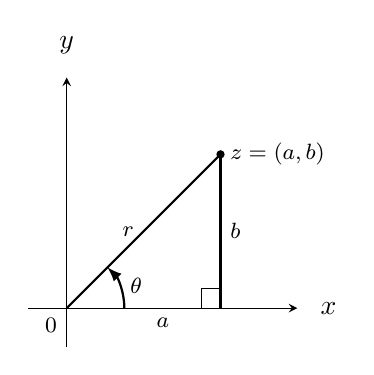
\begin{tikzpicture}
\begin{axis}[disabledatascaling, 
	clip mode=individual, 
    width=5cm, 
    height=5cm, 
    xlabel={$x$}, 
    ylabel={$y$}, 
    axis lines=middle, 
    xtick=\empty, 
    ytick=\empty, 
    xticklabels=\empty, 
    yticklabels=\empty, 
    every axis x label/.style={
      at={(ticklabel* cs:1.05)},
      anchor=west,
    },
    every axis y label/.style={
      at={(ticklabel* cs:1.05)},
      anchor=south,
    },
    domain=-5:5, 
    samples=100, 
    xmin=-0.5, 
    xmax=3, 
    ymin=-0.5, 
    ymax=3]
\draw[thick](0,0)--(2,2);
\fill[black] (2,2) circle (1.5pt);
\draw[thick,-latex] (0.75,0) arc [start angle=0,end angle=45,radius=0.75] node[right,text=black,font=\footnotesize,midway]{$\theta$};
\draw[thick](2,0)--(2,2);
\draw (1.75,0)--(1.75,0.25)--(2,0.25);
\node[below left,font=\footnotesize] at (0,0){$0$};
\node[below,font=\footnotesize] at (1.25,0){$a$};
\node[right,font=\footnotesize] at (2,1){$b$};
\node[left,font=\footnotesize] at (1,1){$r$};
\node[right,font=\footnotesize] at (2,2){$z=(a,b)$};
\end{axis} 
\end{tikzpicture}

	\caption{\label{fig:033977}}
\end{wrapfigure}
If $z \neq 0$, the angle $\theta$ shown in Figure~\ref{fig:033977} is called an \textbf{argument}\index{argument} of $z$ and is denoted
\begin{equation*}
\theta = \func{arg} z
\end{equation*} 
This angle is not unique ($\theta + 2\pi k$ would do as well for any \newline $k = 0, \pm 1, \pm 2, \dots$ ). However, there is only one argument $\theta$ in the range $-\pi < \theta \leq \pi$, and this is sometimes called the \textbf{principal argument}\index{principal argument} of $z$.

Returning to Figure~\ref{fig:033977}, we find that the real and imaginary parts $a$ and $b$ of $z$ are related to $r$ and $\theta$ by
\begin{align*}
a &= r \cos \theta \\
b &= r \sin \theta
\end{align*}
Hence the complex number $z = a + bi$ has the form
\begin{equation*}
z = r(\cos \theta + i \sin \theta) \quad r = |z|, \theta = \func{arg}(z)
\end{equation*}
The combination $\cos \theta + i \sin \theta$ is so important that a special notation is used:
\begin{equation*}
e^{i\theta} = \cos \theta + i \sin \theta
\end{equation*}
is called \textbf{Euler's formula}\index{Euler's formula} after the great Swiss mathematician Leonhard Euler (1707--1783)\index{Euler, Leonhard}. With this notation, $z$ is written
\begin{equation*}
z = r e^{i \theta} \quad r = |z|, \theta = \func{arg}(z)
\end{equation*}
This is a \textbf{polar form} of the complex number $z$. Of course it is not unique, because the argument can be changed by adding a multiple of $2\pi$.


\begin{example}{}{033987}
Write $z_{1} = -2 + 2i$ and $z_{2} = -i$ in polar form.


\begin{solution}
\begin{wrapfigure}[7]{l}{5cm}
	\centering
	
\begin{tikzpicture}
\begin{axis}[disabledatascaling, 
	clip mode=individual, 
    width=5cm, 
    height=5cm, 
    xlabel={$x$}, 
    ylabel={$y$}, 
    axis lines=middle, 
    xtick=\empty, 
    ytick=\empty, 
    xticklabels=\empty, 
    yticklabels=\empty, 
    every axis x label/.style={
      at={(ticklabel* cs:1.05)},
      anchor=west,
    },
    every axis y label/.style={
      at={(ticklabel* cs:1.05)},
      anchor=south,
    },
    domain=-5:5, 
    samples=100, 
    xmin=-2.1, 
    xmax=2.1, 
    ymin=-2.1, 
    ymax=2.1]
\draw[dkgreenvect,thick](0,0)--(-2,2);
\draw[dkgreenvect,thick](0,0)--(0,-1);
\draw[-latex] (0.75,0) arc [start angle=0,end angle=135,radius=0.75] node [right, text=black,font=\footnotesize,midway]{$\theta_1$};
\draw[-latex] (0.5,0) arc [start angle=0,end angle=270,radius=0.5] node [left, text=black,font=\footnotesize,pos=0.95]{$\theta_2$};
\fill[black] (-2,2) circle (1.5pt);
\fill[black] (0,-1) circle (1.5pt);
\node[below right,font=\footnotesize] at (0,0){$0$};
\node[above,font=\footnotesize] at (-2,2){$z_1=-2+2i$};
\node[right,font=\footnotesize] at (0,-1){$z_2=-i$};
\end{axis} 
\end{tikzpicture}

	\caption{\label{fig:033996}}	
\end{wrapfigure}

\setlength{\rightskip}{0pt plus 200pt}
The two numbers are plotted in the complex plane in Figure~\ref{fig:033996}. The absolute values are
\begin{align*}
r_1 &= |-2 + 2i| = \sqrt{(-2)^2 + 2^2} = 2\sqrt{2}\\
r_2 &= |-i| = \sqrt{0^2 + (-1)^2} = 1
\end{align*}
By inspection of Figure~\ref{fig:033996}, arguments of $z_{1}$ and $z_{2}$ are
\begin{align*}
\theta_1 &= \func{arg}(-2+2i) = \frac{3\pi}{4}\\
\theta_2 &= \func{arg}(-i) = \frac{3\pi}{2}
\end{align*}
The corresponding polar forms are $z_{1} = -2 + 2i = 2\sqrt{2} e^{3\pi i/4}$
 and $z_{2} = -i = e^{3\pi i/2}$. Of course, we could have taken the argument $-\frac{\pi}{2}$ for $z_{2}$ and obtained the polar form $z_{2} = e^{-\pi i/2}$.
\end{solution}
\end{example}

In Euler's formula $e^{i\theta}= \cos \theta + i \sin \theta$, the number $e$ is the familiar constant $e = 2.71828\dots$  from calculus. The reason for using $e$ will not be given here; the reason why $\cos \theta + i \sin \theta$ is written as an \textit{exponential} function of $\theta$ is that the \textbf{law of exponents}\index{law of exponents} holds:
\begin{equation*}
e^{i\theta} \cdot e^{i\phi} = e^{i (\theta + \phi)}
\end{equation*}
where $\theta$ and $\phi$ are any two angles. In fact, this is an immediate consequence of the addition identities for $\sin(\theta + \phi)$ and $\cos(\theta + \phi)$:
\newpage
\begin{align*}
e^{i\theta} e^{i\phi} &= (\cos \theta + i \sin \theta) (\cos \phi + i \sin \phi) \\
&= (\cos \theta \cos \phi - \sin \theta \sin \phi) + i (\cos \theta \sin \phi + \sin \theta \cos \phi) \\
&= \cos (\theta +  \phi) +i \sin (\theta + \phi) \\
& =e^{i (\theta + \phi)}
\end{align*}
This is analogous to the rule $e^{a}e^{b} = e^{a+b}$, which holds for real numbers $a$ and $b$, so it is not unnatural to use the exponential notation $e^{i\theta}$ for the expression $\cos \theta + i \sin \theta$. In fact, a whole theory exists wherein functions such as $e^{z}$, $\sin z$, and $\cos z$ are studied, where $z$ is a \textit{complex}
 variable. Many deep and beautiful theorems can be proved in this 
theory, one of which is the so-called fundamental theorem of algebra 
mentioned later (Theorem~\ref{thm:034196}). We shall not pursue this here.


The geometric description of the multiplication of two complex numbers follows from the law of exponents.


\begin{theorem}{Multiplication Rule}{034029}
If $z_{1} = r_{1}e^{i{\theta}_1}$ and $z_{2} = r_{2}e^{i{\theta}_2}$ are complex numbers in polar form, then
\begin{equation*}
z_1z_2 = r_1r_2e^{i (\theta_1 + \theta_2)}
\end{equation*}\index{multiplication rule}
\vspace*{-2em}
\end{theorem}

\noindent In other words, to multiply two complex
 numbers, simply multiply the absolute values and add the arguments. 
This simplifies calculations considerably, particularly when we observe 
that it is valid for \textit{any} arguments $\theta_{1}$ and $\theta_{2}$.


\begin{example}{}{034047}
Multiply $(1-i)(1+\sqrt{3}i)$ in two ways.


\begin{solution}
\begin{wrapfigure}[8]{l}{5cm}
	\centering
	
\begin{tikzpicture}
\begin{axis}[disabledatascaling, 
	clip mode=individual, 
    width=5cm, 
    height=5cm, 
    xlabel={$x$}, 
    ylabel={$y$}, 
    axis lines=middle, 
    xtick=\empty, 
    ytick=\empty, 
    xticklabels=\empty, 
    yticklabels=\empty, 
    every axis x label/.style={
      at={(ticklabel* cs:1.05)},
      anchor=west,
    },
    every axis y label/.style={
      at={(ticklabel* cs:1.05)},
      anchor=south,
    },
    domain=-5:5, 
    samples=100, 
    xmin=-0.25, 
    xmax=3, 
    ymin=-2.1, 
    ymax=2.5]
\draw[dkgreenvect,thick](0,0)--(1,1.73);
\draw[-latex] (0.5,0) arc [start angle=0,end angle=60,radius=0.5] node [right, text=black,font=\scriptsize,pos=0.8]{$\frac{\pi}{3}$};
\draw[dkgreenvect,thick](0,0)--(1,-1);
\draw[-latex] (0.75,0) arc [start angle=0,end angle=-45,radius=0.75] node [right, text=black,font=\scriptsize,midway]{$-\frac{\pi}{4}$};
\draw[dkgreenvect,thick](0,0)--(2.73,0.73);
\draw[-latex] (2,0) arc [start angle=0,end angle=15,radius=2] node [right, text=black,font=\scriptsize,midway]{$\frac{\pi}{12}$};
\fill[dkgreenvect] (1,1.73) circle (1.5pt);
\fill[dkgreenvect] (1,-1) circle (1.5pt);
\fill[dkgreenvect] (2.73,0.73) circle (1.5pt);
\node[below left,font=\scriptsize] at (0,0){$0$};
\node[above,font=\scriptsize] at (1,1.73){$1+\sqrt{3}i$};
\node[below,font=\scriptsize] at (1,-1){$1-i$};
\node[above,font=\scriptsize] at (2.5,0.73){$(1-i)(1+\sqrt{3}i)$};
\end{axis} 
\end{tikzpicture}

	\caption{\label{fig:034054}}
\end{wrapfigure}
	
\setlength{\rightskip}{0pt plus 200pt}
  We have $|1 - i| = \sqrt{2}$ and $|1 + \sqrt{3}i| = 2$ so, from Figure~\ref{fig:034054},
\begin{align*}
& 1-i = \sqrt{2} e^{-i\pi /4} \\
& 1+ \sqrt{3}i = 2e^{i\pi /3}
\end{align*}

Hence, by the multiplication rule,
\begin{align*}
(1-i)(1+\sqrt{3}i) &= (\sqrt{2} e^{-i\pi /4})(2e^{i\pi /3}) \\
&= 2\sqrt{2} e^{i(-\pi/4 + \pi/3)} \\
&= 2 \sqrt{2} e^{i\pi/12}
\end{align*}

This gives the required product in polar form. Of course, direct multiplication gives $(1 - i)(1 + \sqrt{3}i) = (\sqrt{3} + 1) + (\sqrt{3} - 1)i$. Hence, equating real and imaginary parts gives the formulas $\cos (\frac{\pi}{12}) = \frac{\sqrt{3}+1}{2\sqrt{2}}$ and $\sin (\frac{\pi}{12}) = \frac{\sqrt{3}-1}{2\sqrt{2}}$.
\end{solution}
\end{example}

\subsection*{Roots of Unity}

If a complex number $z = re^{i\theta}$ is given in polar form, the powers assume a particularly simple form. In fact, $z^{2} = (re^{i\theta})(re^{i\theta}) = r^{2}e^{2i\theta}$, $z^{3} = z^{2} \cdot z = (r^{2}e^{2i\theta})(re^{i\theta}) = r^{3}e^{3i\theta}$, and so on. Continuing in this way, it follows by induction that the following theorem holds for any positive integer $n$. The name honours Abraham De Moivre (1667--1754).\index{complex number!roots of unity}\index{De Moivre, Abraham}\index{roots of unity}


\begin{theorem}{De Moivre's Theorem}{034080}
If $\theta$ is any angle, then $(e^{i\theta})^{n} = e^{in\theta}$ holds for all integers $n$.\index{De Moivre's Theorem}
\end{theorem}

\begin{proof}
The case $n > 0$ has been discussed, and the reader can verify the result for $n = 0$. To derive it for $n < 0$, first observe that
\begin{equation*}
\mbox{if } \quad z = re^{i\theta}\neq 0 \quad \mbox{ then } \quad z^{-1} = \frac{1}{r}~e^{-i\theta}
\end{equation*}
In fact, $(re^{i\theta})(\frac{1}{r} e^{-i\theta}) = 1e^{i0} = 1$ by the multiplication rule. Now assume that $n$ is negative and write it as $n = -m$, $m > 0$. Then
\begin{equation*}
(re^{i\theta})^n = [(re^{i\theta})^{-1}]^m = (\frac{1}{r}~e^{-i\theta})^m = r^{-m} e^{i(-m\theta)}=r^ne^{in\theta}
\end{equation*}
If $r = 1$, this is De Moivre's theorem for negative $n$.
\end{proof}

\begin{example}{}{034096}
\begin{wrapfigure}{l}{5cm}
        \vspace*{-1.5em}
	\centering
	
\begin{tikzpicture}%[scale=0.75]
\begin{axis}[disabledatascaling, 
	clip mode=individual, 
    width=5cm, 
    height=5cm, 
    xlabel={$x$}, 
    ylabel={$y$}, 
    axis lines=middle, 
    xtick=\empty, 
    ytick=\empty, 
    xticklabels=\empty, 
    yticklabels=\empty, 
    every axis x label/.style={
      at={(ticklabel* cs:1.05)},
      anchor=west,
    },
    every axis y label/.style={
      at={(ticklabel* cs:1.05)},
      anchor=south,
    },
    domain=-5:5, 
    samples=100, 
    xmin=-2, 
    xmax=2, 
    ymin=-0.5, 
    ymax=2]
\draw[dkgreenvect,thick](0,0)--(-1,1.73);
\draw[-latex] (0.75,0) arc [start angle=0,end angle=120,radius=0.75] node [right, text=black,font=\scriptsize,midway]{$\frac{2\pi}{3}$};
\fill[dkgreenvect] (-1,1.73) circle (1.5pt);
\node[below left,font=\scriptsize] at (0,0){$0$};
\node[above,font=\scriptsize] at (-1,1.73){$-1+\sqrt{3}i$};
\node[below left,font=\scriptsize] at (-0.5,0.865){$2$};
\end{axis} 
\end{tikzpicture}

	\caption{\label{fig:034105}}
\end{wrapfigure}

\setlength{\rightskip}{0pt plus 200pt}
Verify that $(-1+\sqrt{3}i)^3 = 8$.

\begin{solution}
  We have $| -1 + \sqrt{3}i| =2$, so $-1 + \sqrt{3}i = 2e^{2\pi i /3}$ (see Figure~\ref{fig:034105}). Hence De Moivre's theorem gives
\begin{equation*}
(-1+\sqrt{3}i)^3 = (2e^{2\pi i /3})^3 = 8e^{3(2\pi i /3)} = 8e^{2\pi i} = 8
\end{equation*}
\vspace{3em}
\end{solution}
\end{example}

De Moivre's theorem can be used to find $n$th roots of complex numbers where $n$ is positive. The next example illustrates this technique.


\begin{example}{}{034107}
Find the cube roots of unity; that is, find all complex numbers $z$ such that $z^{3} = 1$.


\begin{solution}
  First write $z = re^{i\theta}$ and $1 = 1e^{i0}$ in polar form. We must use the condition $z^{3} = 1$ to determine $r$ and $\theta$. Because $z^{3} = r^{3}e^{3i\theta}$ by De Moivre's theorem, this requirement becomes
\begin{equation*}
r^3 e^{3i\theta} = 1 e^{0i}
\end{equation*}
These two complex numbers are equal, so
 their absolute values must be equal and the arguments must either be 
equal or differ by an integral multiple of $2\pi$:
\begin{align*}
r^3 & = 1 \\
3 \theta &= 0 +2k\pi, \quad k \mbox{ some integer} 
\end{align*}
Because $r$ is real and positive, the condition $r^{3} = 1$ implies that $r = 1$. However,
\begin{equation*}
\theta = \frac{2k\pi}{3}, \quad k \mbox{ some integer}
\end{equation*}
\begin{wrapfigure}[8]{l}{5cm}
        \vspace*{-2em}
	\centering
	
\begin{tikzpicture}
\begin{axis}[disabledatascaling, 
	clip mode=individual, 
    width=5cm, 
    height=5cm, 
    xlabel={$x$}, 
    ylabel={$y$}, 
    axis lines=middle, 
    xtick={-5,-4,...,5}, 
    ytick={-5,-4,...,5}, 
    xticklabels=\empty, 
    yticklabels=\empty, 
    every axis x label/.style={
      at={(ticklabel* cs:1.05)},
      anchor=west,
    },
    every axis y label/.style={
      at={(ticklabel* cs:1.05)},
      anchor=south,
    },
    domain=-5:5, 
    samples=100, 
    xmin=-1.5, 
    xmax=1.5, 
    ymin=-1.5, 
    ymax=1.5]
\draw (0,0) circle (1); 
\draw[-latex] (0.5,0) arc [start angle=0,end angle=120,radius=0.5] node [right, text=black,font=\footnotesize,midway]{$\frac{2\pi}{3}$};
\draw[dkgreenvect,thick](0,0)--(-0.5,0.866);
\draw[-latex] (0.25,0) arc [start angle=0,end angle=240,radius=0.25] node [left, text=black,font=\footnotesize,pos=0.95]{$\frac{4\pi}{3}$};
\draw[dkgreenvect,thick](0,0)--(-0.5,-0.866);
\fill[black] (1,0) circle (1.5pt);
\fill[black] (-0.5,0.866) circle (1.5pt);
\fill[black] (-0.5,-0.866) circle (1.5pt);
\node[below right,font=\footnotesize] at (0,0){$0$};
\node[below right,font=\footnotesize] at (1,0){$1$};
\node[above left,font=\footnotesize] at (-0.5,0.866){$-\frac{1}{2}+\frac{\sqrt{3}}{2}i$};
\node[below left,font=\footnotesize] at (-0.5,-0.866){$-\frac{1}{2}-\frac{\sqrt{3}}{2}i$};
\end{axis} 
\end{tikzpicture}

	\caption{\label{fig:034128}}
\end{wrapfigure}
\setlength{\rightskip}{0pt plus 200pt}
seems at first glance to yield infinitely many different angles for $z$. However, choosing $k = 0, 1, 2$ gives three possible arguments $\theta$ (where $0 \leq \theta < 2\pi$), and the corresponding roots are
\begin{align*}
1e^{0i} & = 1 \\
1e^{2\pi i/3} & = -\frac{1}{2} + \frac{\sqrt{3}}{2} i \\
1e^{4\pi i/3} & = -\frac{1}{2} - \frac{\sqrt{3}}{2} i
\end{align*}
These are displayed in Figure~\ref{fig:034128}. All other values of $k$
 yield values of $\theta$ that differ from one of these by a multiple of $2\pi$---and
 so do not give new roots. Hence we have found all the roots.
\end{solution}
\end{example}

The same type of calculation gives all complex $n$\textbf{th roots of unity}; that is, all complex numbers $z$ such that $z^n = 1$. As before, write $1 = 1e^{0i}$ and
\begin{equation*}
z = re^{i\theta}
\end{equation*}
in polar form. Then $z^n = 1$ takes the form
\begin{equation*}
r^ne^{ni\theta} = 1e^{0i}
\end{equation*}
using De Moivre's theorem. Comparing absolute values and arguments yields
\begin{align*}
r^n &= 1 \\
n\theta & = 0 + 2k\pi, \quad k \mbox{ some integer}
\end{align*}
Hence $r = 1$, and the $n$ values
\begin{equation*}
\theta = \frac{2k\pi}{n}, \quad k=0, 1, 2, \dots, n-1
\end{equation*}
of $\theta$ all lie in the range $0 \leq \theta < 2\pi$. As in Example~\ref{exa:034107}, \textit{every} choice of $k$ yields a value of $\theta$ that differs from one of these by a multiple of $2\pi$, so these give the arguments of \textit{all} the possible roots.


\begin{theorem}{$n$th Roots of Unity}{034138}
If $n \geq 1$ is an integer, the $n$th roots of unity (that is, the solutions to $z^n = 1$) are given by
\begin{equation*}
z = e^{2\pi ki/n}, \quad k = 0, 1, 2, \dots, n-1
\end{equation*}\index{$n$th roots of unity}
\vspace*{-2em}
\end{theorem}

\begin{wrapfigure}[6]{l}{5cm}
        \vspace*{-1em}
	\centering
	
\begin{tikzpicture}[scale=0.9]
\begin{axis}[disabledatascaling, 
	clip mode=individual, 
    width=5cm, 
    height=5cm, 
    xlabel={$x$}, 
    ylabel={$y$}, 
    axis lines=middle, 
    xtick={-5,-4,...,5}, 
    ytick={-5,-4,...,5}, 
    xticklabels=\empty, 
    yticklabels=\empty, 
    every axis x label/.style={
      at={(ticklabel* cs:1.05)},
      anchor=west,
    },
    every axis y label/.style={
      at={(ticklabel* cs:1.05)},
      anchor=south,
    },
    domain=-5:5, 
    samples=100, 
    xmin=-1.5, 
    xmax=1.5, 
    ymin=-1.5, 
    ymax=1.5]
\draw (0,0) circle (1); 
\draw[dkgreenvect,thick](0,0)--(1,0);
\draw[dkgreenvect,thick](0,0)--(0.309,0.951);
\draw[dkgreenvect,thick](0,0)--(-0.809,0.588);
\draw[dkgreenvect,thick](0,0)--(-0.809,-0.588);
\draw[dkgreenvect,thick](0,0)--(0.309,-0.951);


\fill[black] (1,0) circle (1.5pt);
\fill[black] (0.309,0.951) circle (1.5pt);
\fill[black] (-0.809,0.588) circle (1.5pt);
\fill[black] (-0.809,-0.588) circle (1.5pt);
\fill[black] (0.309,-0.951) circle (1.5pt);

\node[below right,font=\footnotesize] at (0,0){$0$};
\node[above right,font=\footnotesize] at (0.9,0){$1=e^{0i}$};
\node[above right,font=\footnotesize] at (0.309,0.951){$e^{2\pi i/5}$};
\node[left,font=\footnotesize] at (-0.809,0.588){$e^{4\pi i/5}$};
\node[below left,font=\footnotesize] at (-0.809,-0.588){$e^{6\pi i/5}$};
\node[below right,font=\footnotesize] at (0.309,-0.951){$e^{8\pi i/5}$};
\end{axis} 
\end{tikzpicture}

	\caption{\label{fig:034146}}
\end{wrapfigure}

\noindent The $n$th roots of unity can be found geometrically as the points on the unit circle that cut the circle into $n$ equal sectors, starting at $1$. The case $n = 5$ is shown in Figure~\ref{fig:034146}, where the five fifth roots of unity are plotted.

\vspace{2em}

The method just used to find the $n$th roots of unity works equally well to find the $n$th roots of any complex number in polar form. We give one example.

\begin{example}{}{034148}
Find the fourth roots of $\sqrt{2} + \sqrt{2}i$.


\begin{solution}
  First write $\sqrt{2} + \sqrt{2}i = 2e^{\pi i/4}$ in polar form. If $z = re^{i\theta}$ satisfies $z^{4} = \sqrt{2} + \sqrt{2}i$, then De Moivre's theorem gives
\begin{equation*}
r^4e^{i(4\theta)} = 2e^{\pi i/4}
\end{equation*}
Hence $r^{4} = 2$ and $4\theta = \frac{\pi}{4} + 2k\pi$, $k$ an integer. We obtain four distinct roots (and hence all) by
\begin{equation*}
r = \sqrt[4]{2}, \quad \theta = \frac{\pi}{16} = \frac{2k\pi}{16}, k=0, 1, 2, 3
\end{equation*}
Thus the four roots are
\begin{equation*}
\sqrt[4]{2} e^{\pi i/16} \quad  \sqrt[4]{2} e^{9\pi i/16} \quad \sqrt[4]{2} e^{17 \pi i/16} \quad \sqrt[4]{2} e^{25\pi i/16}
\end{equation*}
Of course, reducing these roots to the form $a + bi$ would require the computation of $\sqrt[4]{2}$
 and the sine and cosine of the various angles.
\end{solution}
\end{example}

An expression of the form $ax^{2} + bx + c$, where the coefficients $a \neq 0$, $b$, and $c$ are real numbers, is called a \textbf{real quadratic}\index{real quadratic}. A complex number $u$ is called a \textbf{root}\index{root!of the quadratic} of the quadratic if $au^{2} + bu + c = 0$. The roots are given by the famous \textbf{quadratic formula}\index{quadratic formula}:
\begin{equation*}
u = \frac{-b \pm \sqrt{b^2 - 4ac}}{2a}
\end{equation*}
The quantity $d = b^{2} - 4ac$ is called the \textbf{discriminant}\index{discriminant} of the quadratic $ax^{2} + bx + c$, and there is no real root if and only if $d < 0$. In this case the quadratic is said to be \textbf{irreducible}\index{irreducible}. Moreover, the fact that $d < 0$ means that $\sqrt{d} = i\sqrt{|d|}$, so the two (complex) roots are conjugates of each other:
\begin{equation*}
u = \frac{1}{2a}(-b+i\sqrt{|d|}) \quad \mbox{ and } \quad \overline{u} = \frac{1}{2a}(-b-i\sqrt{|d|})
\end{equation*}
The converse of this is true too: Given any nonreal complex number $u$, then $u$ and $\overline{u}$
 are the roots of some real irreducible quadratic. Indeed, the quadratic
\begin{equation*}
x^2 - (u + \overline{u})x + u \overline{u} = (x-u)(x-\overline{u})
\end{equation*}
has real coefficients ($u\overline{u} = |u|^{2}$ and $u + \overline{u}$
 is twice the real part of $u$) and so is irreducible because its roots $u$ and $\overline{u}$
 are not real.


\begin{example}{}{034182}
Find a real irreducible quadratic with $u = 3 - 4i$ as a root.


\begin{solution}
  We have $u + \overline{u} = 6$ and $|u|^{2} = 25$, so $x^{2} - 6x + 25$ is irreducible with $u$ and $\overline{u} = 3 + 4i$ as roots.
\end{solution}
\end{example}

\subsection*{Fundamental Theorem of Algebra}

As we mentioned earlier, the complex 
numbers are the culmination of a long search by mathematicians to find a
 set of numbers large enough to contain a root of every polynomial. The 
fact that the complex numbers have this property was first proved by 
Gauss in 1797 when he was 20 years old. The proof is omitted.


\begin{theorem}{Fundamental Theorem of Algebra}{034196}
Every polynomial of positive degree with complex coefficients has a complex root.
\end{theorem}

\noindent If $f(x)$ is a polynomial with complex coefficients, and if $u_{1}$ is a root, then the factor theorem (Section~\ref{sec:6_5}) asserts that
\begin{equation*}
f(x) = (x-u_1)g(x)
\end{equation*}
where $g(x)$ is a polynomial with complex coefficients and with degree one less than the degree of $f(x)$. Suppose that $u_{2}$ is a root of $g(x)$, again by the fundamental theorem. Then $g(x) = (x - u_{2})h(x)$, so
\begin{equation*}
f(x) = (x-u_1)(x-u_2)h(x)
\end{equation*}
This process continues until the last polynomial to appear is linear. Thus $f(x)$ has been expressed as a product of linear factors. The last of these factors can be written in the form $u(x - u_{n})$, where $u$ and $u_{n}$ are complex (verify this), so the fundamental theorem takes the following form.


\begin{theorem}{}{034210}
Every complex polynomial $f(x)$ of degree $n \geq 1$ has the form
\begin{equation*}
f(x) = u(x-u_1)(x-u_2)\cdots (x-u_n)
\end{equation*}
where $u, u_{1}, \dots, u_{n}$ are complex numbers and $u \neq 0$. The numbers $u_{1}, u_{2}, \dots, u_{n}$ are the roots of $f(x)$ (and need not all be distinct), and $u$ is the coefficient of $x^{n}$.
\end{theorem}

\noindent This form of the fundamental theorem, when applied to a polynomial $f(x)$ with \textit{real} coefficients, can be used to deduce the following result.


\begin{theorem}{}{034221}
Every polynomial $f(x)$ of positive 
degree with real coefficients can be factored as a product of linear and
 irreducible quadratic factors.
\end{theorem}

\noindent In fact, suppose $f(x)$ has the form
\begin{equation*}
f(x) = a_nx^n + a_{n-1}x^{n-1} + \cdots + a_1x + a_0
\end{equation*}
where the coefficients $a_{i}$ are real. If $u$ is a complex root of $f(x)$, then we claim first that $\overline{u}$
 is also a root. In fact, we have $f(u) = 0$, so
\begin{align*}
0 = \overline{0} = \overline{f(u)} & = \overline{a_nu^n + a_{n-1}u^{n-1} + \cdots + a_1u + a_0 } \\
& = \overline{a_nu^n} + \overline{a_{n-1}u^{n-1}} + \cdots + \overline{a_1u} + \overline{a_0 } \\
& = \overline{a}_n\overline{u}^n + \overline{a}_{n-1}\overline{u}^{n-1} + \cdots + \overline{a}_1\overline{u} + \overline{a}_0 \\
& = a_n\overline{u}^n + a_{n-1}\overline{u}^{n-1} + \cdots + a_1\overline{u} + a_0 \\
&= f(\overline{u})
\end{align*}
where $\overline{a}_i = a_i$
 for each $i$ because the coefficients $a_{i}$ are real. Thus if $u$ is a root of $f(x)$, so is its conjugate $\overline{u}$. Of course some of the roots of $f(x)$ may be real (and so equal their conjugates), but the nonreal roots come in pairs, $u$ and $\overline{u}$. By Theorem~\ref{thm:034221}, we can thus write $f(x)$ as a product:
\begin{equation}\label{eq:complexproduct}
f(x) = a_n(x-r_1)\cdots(x-r_k)(x-u_1)(x-\overline{u}_1)\cdots (x-u_m)(x-\overline{u}_m)
\end{equation}
where $a_{n}$ is the coefficient of $x^{n}$ in $f(x)$; $r_{1}, r_{2}, \dots , r_{k}$ are the real roots; and $u_{1}, \overline{u}_{1}, u_{2}, \overline{u}_{2}, \dots , u_{m}, \overline{u}_{m}$ are the nonreal roots. But the product
\begin{equation*}
(x-u_j)(x-\overline{u}_j) = x^2 - (u_j + \overline{u}_j)x +(u_j \overline{u}_j)
\end{equation*}
is a real irreducible quadratic for each $j$ (see the discussion preceding Example~\ref{exa:034182}). Hence (\ref{eq:complexproduct}) shows that $f(x)$ is a product of linear and irreducible quadratic factors, each with real coefficients. This is the conclusion in Theorem~\ref{thm:034221}.


\section*{Exercises for \ref{chap:appacomplexnumbers}}

\begin{Filesave}{solutions}
\solsection{Appendix~\ref{chap:appacomplexnumbers}}
\end{Filesave}

\begin{multicols}{2}
\begin{ex}
Solve each of the following for the real number $x$.

\begin{exenumerate}
\exitem $x-4i = (2-i)^2$
\exitem $(2+xi)(3-2i) \\ \hspace*{2em}= 12+5i$
\exitem $(2+xi)^2=4$
\exitem $(2+xi)(2-xi)=5$
\end{exenumerate}
\begin{sol}
\begin{enumerate}[label={\alph*.}]
\setcounter{enumi}{1}
\item $x = 3$

\setcounter{enumi}{3}
\item  $x = \pm 1$

\end{enumerate}
\end{sol}
\end{ex}

\columnbreak

\begin{ex}
Convert each of the following to the form $a + bi$.

\begin{exenumerate}
\exitem* $(2-3i)-2(2-3i)+9$
\exitem*  $(3-2i)(1+i)+|3+4i|$
\exitem $\frac{1+i}{2-3i} + \frac{1-i}{-2+3i}$
\exitem $\frac{3-2i}{1-i} + \frac{3-7i}{2-3i}$
\exitem $i^{131}$
\exitem $(2 - i)^{3}$
\exitem $(1 + i)^{4}$
\exitem $(1 - i)^{2}(2 + i)^{2}$
\exitem* $\frac{3\sqrt{3}-i}{\sqrt{3}+i} + \frac{\sqrt{3}+7i}{\sqrt{3}-i}$
\end{exenumerate}
\begin{sol}
\begin{enumerate}[label={\alph*.}]
\setcounter{enumi}{1}
\item  $10 + i$

\setcounter{enumi}{3}
\item $\frac{11}{26} + \frac{23}{26}i$


\setcounter{enumi}{5}
\item $ 2 - 11i$

\setcounter{enumi}{7}
\item  $8 - 6i$

\end{enumerate}
\end{sol}
\end{ex}

\begin{ex}
In each case, find the complex number $z$.

\begin{exenumerate}
\exitem $ iz - (1 + i)^{2} = 3 - i$
\exitem* $(i + z) - 3i(2 - z) = iz + 1$
\exitem $z^{2} = -i$
\exitem $z^{2} = 3 - 4i$
\exitem $z(1+i) = \overline{z} + (3+2i)$
\exitem* $z(2-i) = (\overline{z}+1)(1+i)$
\end{exenumerate}
\begin{sol}
\begin{enumerate}[label={\alph*.}]
\setcounter{enumi}{1}
\item $\frac{11}{5} + \frac{3}{5}i$


\setcounter{enumi}{3}
\item  $\pm(2 - i)$

\setcounter{enumi}{5}
\item $ 1 + i$

\end{enumerate}
\end{sol}
\end{ex}

\begin{ex}
In each case, find the roots of the real quadratic equation.

\begin{exenumerate}
\exitem  $x^{2} - 2x + 3 = 0$
\exitem  $x^{2} - x + 1 = 0$
\exitem $3x^{2} - 4x + 2 = 0$
\exitem  $2x^{2} - 5x + 2 = 0$
\end{exenumerate}
\begin{sol}
\begin{enumerate}[label={\alph*.}]
\setcounter{enumi}{1}
\item $\frac{1}{2} \pm \frac{\sqrt{3}}{2}i$


\setcounter{enumi}{3}
\item  $2$, $\frac{1}{2}$

\end{enumerate}
\end{sol}
\end{ex}

\begin{ex}
Find all numbers $x$ in each case.

\begin{exenumerate}
\exitem $x^{3} = 8$
\exitem $x^{3} = -8$
\exitem  $x^{4} = 16$
\exitem  $x^{4} = 64$
\end{exenumerate}
\begin{sol}
\begin{enumerate}[label={\alph*.}]
\setcounter{enumi}{1}
\item  $-2$, $1 \pm \sqrt{3}i$


\setcounter{enumi}{3}
\item  $\pm 2\sqrt{2}$, $\pm 2\sqrt{i}$


\end{enumerate}
\end{sol}
\end{ex}

\begin{ex}
In each case, find a real quadratic with $u$ as a root, and find the other root.

\begin{exenumerate}
\exitem  $u = 1 + i$
\exitem  $u = 2 - 3i$
\exitem $u = -i$
\exitem $u = 3 - 4i$
\end{exenumerate}
\begin{sol}
\begin{enumerate}[label={\alph*.}]
\setcounter{enumi}{1}
\item  $x^{2} - 4x + 13$; $2 + 3i$

\setcounter{enumi}{3}
\item  $x^{2} - 6x + 25$; $3 + 4i$

\end{enumerate}
\end{sol}
\end{ex}

\begin{ex}
Find the roots of $x^{2} - 2\cos \theta x + 1 = 0$, $\theta$ any angle.
\end{ex}

\begin{ex}
Find a real polynomial of degree $4$ with $2 - i$ and $3 - 2i$ as roots.

\begin{sol}
$x^{4} - 10x^{3} + 42x^{2} - 82x + 65$
\end{sol}
\end{ex}

\begin{ex}
Let $\func{re }z$ and $\func{im }z$ denote, respectively, the real and imaginary parts of $z$. Show that:

\begin{exenumerate}
\exitem $\func{im}(iz) = \func{re }z$
\exitem $\func{re}(iz) = -\func{im }z$
\exitem $z + \overline{z} = 2 \func{re}z$
\exitem $z - \overline{z} = 2i \func{im} z$
\exitem* $\func{re}(z + w) = \func{re }z + \func{re }w$, and $\func{re}(tz) = t \cdot \func{re }z$ if $t$ is real
\exitem* $\func{im}(z + w) = \func{im }z + \func{im }w$, and $\func{im}(tz) = t \cdot \func{im }z$ if $t$ is real
\end{exenumerate}
\end{ex}

\columnbreak 
\begin{ex}
In each case, show that $u$ is a root of the quadratic equation, and find the other root.\index{complex number!root of the quadratic}

\begin{exenumerate}
\exitem* $x^{2} - 3ix + (-3 + i) = 0$; $u = 1 + i$
\exitem* $x^{2} + ix - (4 - 2i) = 0$; $u = -2$
\exitem* $x^{2} - (3 - 2i)x + (5 - i) = 0$; $u = 2 - 3i$
\exitem* $x^{2} + 3(1 - i)x - 5i = 0$; $u = -2 + i$
\end{exenumerate}
\begin{sol}
\begin{enumerate}[label={\alph*.}]
\setcounter{enumi}{1}
\item  $(-2)^{2} + 2i - (4 - 2i) = 0$; $2 - i$

\setcounter{enumi}{3}
\item  $(-2 + i)^{2} + 3(1 - i)(-1 + 2i) - 5i = 0$; $-1 + 2i$

\end{enumerate}
\end{sol}
\end{ex}

\begin{ex}
Find the roots of each of the following complex quadratic equations.

\begin{exenumerate}
\exitem $x^{2} + 2x + (1 + i) = 0$
\exitem  $x^{2} - x + (1 - i) = 0$
\exitem* $x^{2} - (2 - i)x + (3 - i) = 0$
\exitem* $x^{2} - 3(1 - i)x - 5i = 0$
\end{exenumerate}
\begin{sol}
\begin{enumerate}[label={\alph*.}]
\setcounter{enumi}{1}
\item  $-i$, $1 + i$

\setcounter{enumi}{3}
\item  $2 - i$, $1 - 2i$

\end{enumerate}
\end{sol}
\end{ex}

\begin{ex}
In each case, describe the graph of the equation (where $z$ denotes a complex number).

\begin{exenumerate}
\exitem $|z| = 1$
\exitem $|z - 1| = 2$
\exitem $z = i \overline{z}$
\exitem $z = -\overline{z}$
\exitem $z = |z|$
\exitem $\func{im }z = m \cdot \func{re }z$, $m$ a real number
\end{exenumerate}
\begin{sol}
\begin{enumerate}[label={\alph*.}]
\setcounter{enumi}{1}
\item  Circle, centre at $1$, radius $2$

\setcounter{enumi}{3}
\item  Imaginary axis

\setcounter{enumi}{5}
\item  Line $y = mx$

\end{enumerate}
\end{sol}
\end{ex}

\begin{ex}
\begin{enumerate}[label={\alph*.}]
\item Verify $|zw| = |z||w|$ directly for $z = a + bi$ and $w = c + di$.

\item Deduce (a) from properties C2 and C6.

\end{enumerate}
\end{ex}

\begin{ex}
Prove that $|z+w| = |z|^2 + |w|^2 + w\overline{z} + \overline{w}z$
 for all complex numbers $w$ and $z$.
\end{ex}

\begin{ex}
If $zw$ is real and $z \neq 0$, show that $w = a \overline{z}$
 for some real number $a$.
\end{ex}

\begin{ex}
If $zw = \overline{z}v$
 and $z \neq 0$, show that $w = uv$ for some $u$ in $\mathbb{C}$  with $|u| = 1$.
\end{ex}

\begin{ex}
Show that $(1 + i)^{n} + (1 - i)^{n}$ is real for all $n$, using property C5.
\end{ex}

\begin{ex}
Express each of the following in polar form (use the principal argument).

\begin{exenumerate}
\exitem $3 - 3i$
\exitem $-4i$
\exitem $-\sqrt{3} + i$
\exitem $-4 + 4\sqrt{3}i$
\exitem $-7i$
\exitem $-6 + 6i$
\end{exenumerate}
\begin{sol}
\begin{enumerate}[label={\alph*.}]
\setcounter{enumi}{1}
\item  $4e^{-\pi i/2}$

\setcounter{enumi}{3}
\item  $8e^{2\pi i/3}$

\setcounter{enumi}{5}
\item  $6\sqrt{2}e^{3\pi i/4}$


\end{enumerate}
\end{sol}
\end{ex}

\columnbreak

\begin{ex}
Express each of the following in the form $a + bi$.

\begin{exenumerate}
\exitem $3e^{\pi i}$
\exitem $e^{7\pi i/3}$
\exitem $2e^{3 \pi i/4}$
\exitem $\sqrt{2}e^{-\pi i/4}$
\exitem $e^{5\pi i/4}$
\exitem $2\sqrt{3}e^{-2\pi i/6}$
\end{exenumerate}
\begin{sol}
\begin{enumerate}[label={\alph*.}]
\setcounter{enumi}{1}
\item  $\frac{1}{2} + \frac{\sqrt{3}}{2} i$

\setcounter{enumi}{3}
\item  $1 - i$

\setcounter{enumi}{5}
\item $\sqrt{3} - 3i$


\end{enumerate}
\end{sol}
\end{ex}

\begin{ex}
Express each of the following in the form $a + bi$.

\begin{exenumerate}
\exitem $(-1 + \sqrt{3}i)^2$
\exitem $(1 + \sqrt{3}i)^{-4}$
\exitem $(1 + i)^8$
\exitem $(1 - i)^{10}$
\exitem $(1 - i)^{6}(\sqrt{3} + i)^{3}$
\exitem $(\sqrt{3} - i)^{9}(2 - 2i)^{5}$
\end{exenumerate}
\begin{sol}
\begin{enumerate}[label={\alph*.}]
\setcounter{enumi}{1}
\item  $-\frac{1}{32} + \frac{\sqrt{3}}{32}i$


\setcounter{enumi}{3}
\item  $-32i$

\setcounter{enumi}{5}
\item  $-2^{16}(1 + i)$

\end{enumerate}
\end{sol}
\end{ex}

\begin{ex}
Use De Moivre's theorem to show that:

\begin{enumerate}[label={\alph*.}]
\item $\cos 2\theta = \cos^{2} \theta - \sin^{2} \theta$; $\sin 2\theta = 2 \cos \theta \sin \theta$

\item $\cos 3\theta = \cos^{3} \theta - 3 \cos \theta \sin^{2} \theta$; \\
$\sin 3\theta = 3 \cos^2 \theta \sin \theta - \sin^3 \theta$

\end{enumerate}
\end{ex}

\begin{ex}
\begin{enumerate}[label={\alph*.}]
\item Find the fourth roots of unity.

\item Find the sixth roots of unity.

\end{enumerate}
\end{ex}

\begin{ex}
Find all complex numbers $z$ such that:

\begin{exenumerate}
\exitem $z^{4} = -1$
\exitem $z^{4} = 2(\sqrt{3}i - 1)$
\exitem $z^{3} = -27i$
\exitem $z^{6} = -64$
\end{exenumerate}
\begin{sol}
\begin{enumerate}[label={\alph*.}]
\setcounter{enumi}{1}
\item $\pm \frac{\sqrt{2}}{2}(\sqrt{3}+i)$, $\pm \frac{\sqrt{2}}{2}(-1 + \sqrt{3}i)$


\setcounter{enumi}{3}
\item  $\pm 2i$, $\pm (\sqrt{3} +i)$, $\pm (\sqrt{3}-i)$


\end{enumerate}
\end{sol}
\end{ex}

\columnbreak
\begin{ex}
If $z = re^{i\theta}$ in polar form, show that:

\begin{exenumerate}
\exitem $\overline{z} = re^{-i\theta}$
\exitem $z^{-1}  = \frac{1}{r} e^{-i\theta}$ if  $z \neq 0 $
\end{exenumerate}
\end{ex}

\begin{ex}
Show that the sum of the $n$th roots of unity is zero. \newline [\textit{Hint:} $1 - z^{n} = (1 - z)(1 + z + z^{2} + \dots  + z^{n-1})$ for any complex number $z$.]
\end{ex}

\begin{ex}
\begin{enumerate}[label={\alph*.}]
\item Let $z_{1}$, $z_{2}$, $z_{3}$, $z_{4}$, and $z_{5}$ be equally spaced around the unit circle. Show that $z_{1} + z_{2} + z_{3} + z_{4} + z_{5} = 0$. [\textit{Hint}: $(1 - z)(1 + z + z^{2} + z^{3} + z^{4}) = 1 - z^{5}$ for any complex number $z$.]

\item Repeat (a) for any $n \geq 2$ points equally spaced around the unit circle.

\item If $|w| = 1$, show that the sum of the roots of $z^n = w$ is zero.

\end{enumerate}
\begin{sol}
\begin{enumerate}[label={\alph*.}]
\setcounter{enumi}{1}
\item  The argument in (a) applies using $\beta = \frac{2\pi}{n}$.
 Then $ 1 + z + \cdots + z^{n-1} = \frac{1-z^n}{1-z}=0$.


\end{enumerate}
\end{sol}
\end{ex}

\begin{ex}
If $z^n$ is real, $n \geq 1$, show that $(\overline{z})^{n}$ is real.
\end{ex}

\begin{ex}
If $\overline{z}^2 = z^{2}$, show that $z$ is real or pure imaginary.
\end{ex}

\begin{ex}
If $a$ and $b$ are \textit{rational} numbers, let $p$ and $q$ denote numbers of the form $a + b\sqrt{2}$. If $p = a + b\sqrt{2}$, define $\tilde{p} = a-b\sqrt{2}$ and $[p] = a^{2} - 2b^{2}$. Show that each of the following holds.

\begin{exenumerate}
\exitem* $a + b\sqrt{2} = a_{1} + b_{1}\sqrt{2}$ only if $a = a_{1}$ and $b = b_{1}$
\exitem $\widetilde{p \pm q} = \tilde{p} \pm \tilde{q}$
\exitem $\widetilde{pq} = \tilde{p}\tilde{q}$
\exitem $[p] = p \tilde{p}$
\exitem $[pq] = [p][q]$
\exitem* If $f(x)$ is a polynomial with rational coefficients and $p = a + b\sqrt{2}$ is a root of $f(x)$, then $\tilde{p}$
 is also a root of $f(x)$.
\end{exenumerate}
\end{ex}

\end{multicols}

